\documentclass[12pt,letterpaper]{article}
\usepackage{graphicx,textcomp}
\usepackage{natbib}
\usepackage{setspace}
\usepackage{fullpage}
\usepackage{color}
\usepackage[reqno]{amsmath}
\usepackage{amsthm}
\usepackage{fancyvrb}
\usepackage{amssymb,enumerate}
\usepackage[all]{xy}
\usepackage{endnotes}
\usepackage{lscape}
\newtheorem{com}{Comment}
\usepackage{float}
\usepackage{hyperref}
\newtheorem{lem} {Lemma}
\newtheorem{prop}{Proposition}
\newtheorem{thm}{Theorem}
\newtheorem{defn}{Definition}
\newtheorem{cor}{Corollary}
\newtheorem{obs}{Observation}
\usepackage[compact]{titlesec}
\usepackage{dcolumn}
\usepackage{tikz}
\usetikzlibrary{arrows}
\usepackage{multirow}
\usepackage{xcolor}
\newcolumntype{.}{D{.}{.}{-1}}
\newcolumntype{d}[1]{D{.}{.}{#1}}
\definecolor{light-gray}{gray}{0.65}
\usepackage{url}
\usepackage{listings}
\usepackage{color}

\definecolor{codegreen}{rgb}{0,0.6,0}
\definecolor{codegray}{rgb}{0.5,0.5,0.5}
\definecolor{codepurple}{rgb}{0.58,0,0.82}
\definecolor{backcolour}{rgb}{0.95,0.95,0.92}

\lstdefinestyle{mystyle}{
	backgroundcolor=\color{backcolour},   
	commentstyle=\color{codegreen},
	keywordstyle=\color{magenta},
	numberstyle=\tiny\color{codegray},
	stringstyle=\color{codepurple},
	basicstyle=\footnotesize,
	breakatwhitespace=false,         
	breaklines=true,                 
	captionpos=b,                    
	keepspaces=true,                 
	numbers=left,                    
	numbersep=5pt,                  
	showspaces=false,                
	showstringspaces=false,
	showtabs=false,                  
	tabsize=2
}
\lstset{style=mystyle}
\newcommand{\Sref}[1]{Section~\ref{#1}}
\newtheorem{hyp}{Hypothesis}

\title{Problem Set 3}
\date{Due: November 13, 2025}
\author{Applied Stats/Quant Methods 1}


\begin{document}
	\maketitle
	\section*{Instructions}
	\begin{itemize}
		\item Please show your work! You may lose points by simply writing in the answer. If the problem requires you to execute commands in \texttt{R}, please include the code you used to get your answers. Please also include the \texttt{.R} file that contains your code. If you are not sure if work needs to be shown for a particular problem, please ask.
	\item Your homework should be submitted electronically on GitHub.
	\item This problem set is due before 23:59 on Thursday November 13, 2025. No late assignments will be accepted.

	\end{itemize}

		\vspace{.25cm}
	
\noindent In this problem set, you will run several regressions and create an add variable plot (see the lecture slides) in \texttt{R} using the \texttt{incumbents\_subset.csv} dataset. Include all of your code.

	\vspace{.5cm}
\section*{Question 1}
\vspace{.25cm}
\noindent We are interested in knowing how the difference in campaign spending between incumbent and challenger affects the incumbent's vote share. 
	\begin{enumerate}
		\item Run a regression where the outcome variable is \texttt{voteshare} and the explanatory variable is \texttt{difflog}.	\vspace{.5cm}
		
			\textbf{code}		
			\begin{verbatim}
				reg1 <- lm(voteshare ~ difflog, data=inc.sub)
				reg1
				summary(reg1) # inspect results
				stargazer(reg1, title = "Difference in campaign 
				spending on incumbent vote share")
			\end{verbatim}
			\newpage
			
			\textbf{Stargazer table}		
			
			% Table created by stargazer v.5.2.3 by Marek Hlavac, Social Policy Institute. E-mail: marek.hlavac at gmail.com
			% Date and time: Thu, Nov 13, 2025 - 20:21:56
			\begin{table}[!htbp] \centering 
				\caption{Difference in campaign spending on incumbent vote share} 
				\label{} 
				\begin{tabular}{@{\extracolsep{5pt}}lc} 
					\\[-1.8ex]\hline 
					\hline \\[-1.8ex] 
					& \multicolumn{1}{c}{\textit{Dependent variable:}} \\ 
					\cline{2-2} 
					\\[-1.8ex] & voteshare \\ 
					\hline \\[-1.8ex] 
					difflog & 0.042$^{***}$ \\ 
					& (0.001) \\ 
					& \\ 
					Constant & 0.579$^{***}$ \\ 
					& (0.002) \\ 
					& \\ 
					\hline \\[-1.8ex] 
					Observations & 3,193 \\ 
					R$^{2}$ & 0.367 \\ 
					Adjusted R$^{2}$ & 0.367 \\ 
					Residual Std. Error & 0.079 (df = 3191) \\ 
					F Statistic & 1,852.791$^{***}$ (df = 1; 3191) \\ 
					\hline 
					\hline \\[-1.8ex] 
					\textit{Note:}  & \multicolumn{1}{r}{$^{*}$p$<$0.1; $^{**}$p$<$0.05; $^{***}$p$<$0.01} \\ 
				\end{tabular} 
			\end{table} 
			
			\textit{Interpretation of regression: The intercept is 0.579031, the regression coefficient with difflog is 0.041666, representing a positive relationship between both variables, it indicates that as difference in campaign spending increases, so does the incumbent's vote share. The p-value is <2e-16, which suggests the probability of obtaining results at least as extreme as those observed, with such a small p-value, we can reject the null hypothesis that there is no relationship between difference in campaign spending an incumbent vote share.}\vspace{.5cm}
		
		\item Make a scatterplot of the two variables and add the regression line. 	\vspace{.5cm}
			
			\textbf{code}		
			\begin{verbatim}
				ggplot(data=inc.sub, aes(x = difflog, y = voteshare)) +
				geom_point(size = 2, shape = 1, color = "navy") +
				geom_smooth(method = lm, color = "red3") +
				labs(title = "Difference in campaign spending on incumbent vote share",
				x = "Difference in campaign spending",
				y = "Incumbent vote share") +
				theme_bw()
			\end{verbatim}
			
			\begin{figure}
				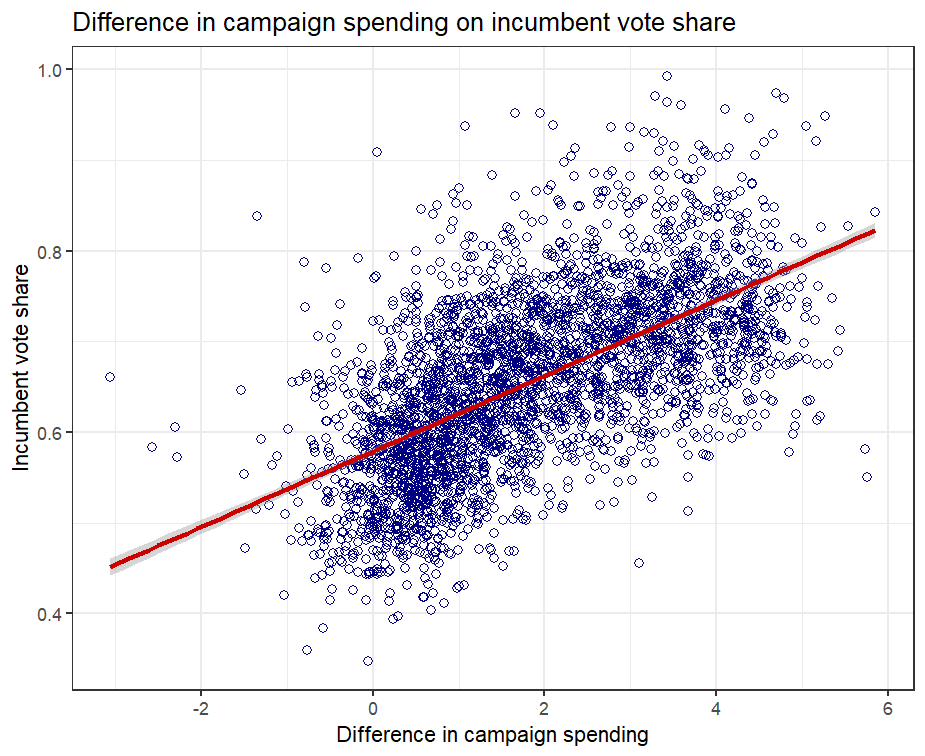
\includegraphics[width=\linewidth]{Rplot1.png}
				\caption{Difference in campaign spending on incumbent vote share.}
				\label{fig:Difference in campaign spending on incumbent vote share}
			\end{figure}
			
			\textit{Interpretation of Figure 1 scatter plot: reflects the findings of the previous regression, a linear, strong, positive relationship between both variables. It reflects a positive correlation between both variables.}\vspace{.5cm}

		
		\item Save the residuals of the model in a separate object.	\vspace{.5cm}
			
			\textbf{code}		
			\begin{verbatim}
				res1 <- resid(reg1)
				res1
			\end{verbatim}

			\textit{Residuals indicate the distance of the values of each observation from the predicted values, which fall on the line of best fit.}\vspace{.5cm}
		
		\item Write the prediction equation.
		
			\textit{The formula for the prediction equation is: y = intercept +(slope*x). Therefore, using the data from the regression, the formula for this question is: incumbent vote share = 0.579031 + (0.041666*difference in campaign spending).}\vspace{.5cm}
			
	\end{enumerate}
	
\newpage

\section*{Question 2}
\noindent We are interested in knowing how the difference between incumbent and challenger's spending and the vote share of the presidential candidate of the incumbent's party are related.	\vspace{.25cm}
	\begin{enumerate}
		\item Run a regression where the outcome variable is \texttt{presvote} and the explanatory variable is \texttt{difflog}.	\vspace{.5cm}
			
			\textbf{code}		
			\begin{verbatim}
				reg2 <- lm(presvote ~ difflog, data=inc.sub)
				reg2
				summary(reg2) # inspect results
				stargazer(reg2, title = "Difference in campaign 
				spending on presidential candidate of the incumbent party vote share")
				
			\end{verbatim}
			
			\textbf{Stargazer table}		
			
			% Table created by stargazer v.5.2.3 by Marek Hlavac, Social Policy Institute. E-mail: marek.hlavac at gmail.com
			% Date and time: Thu, Nov 13, 2025 - 21:53:44
			\begin{table}[!htbp] \centering 
				\caption{Difference in campaign spending on incumbent party's presidential candidate vote share} 
				\label{} 
				\begin{tabular}{@{\extracolsep{5pt}}lc} 
					\\[-1.8ex]\hline 
					\hline \\[-1.8ex] 
					& \multicolumn{1}{c}{\textit{Dependent variable:}} \\ 
					\cline{2-2} 
					\\[-1.8ex] & presvote \\ 
					\hline \\[-1.8ex] 
					difflog & 0.024$^{***}$ \\ 
					& (0.001) \\ 
					& \\ 
					Constant & 0.508$^{***}$ \\ 
					& (0.003) \\ 
					& \\ 
					\hline \\[-1.8ex] 
					Observations & 3,193 \\ 
					R$^{2}$ & 0.088 \\ 
					Adjusted R$^{2}$ & 0.088 \\ 
					Residual Std. Error & 0.110 (df = 3191) \\ 
					F Statistic & 307.715$^{***}$ (df = 1; 3191) \\ 
					\hline 
					\hline \\[-1.8ex] 
					\textit{Note:}  & \multicolumn{1}{r}{$^{*}$p$<$0.1; $^{**}$p$<$0.05; $^{***}$p$<$0.01} \\ 
				\end{tabular} 
			\end{table}
			
			\textit{Interpretation of regression: The intercept is 0.507583, the regression coefficient with difflog is 0.023837, representing a positive relationship between both variables, it indicates that as difference in campaign spending increases, so does the incumbent's party's presidential candidate vote share. The p-value is <2e-16, which suggests the probability of obtaining results at least as extreme as those observed, with such a small p-value, we can reject the null hypothesis that there is no relationship between difference in campaign spending and incumbent's party's presidential candidate's vote share.}
			
			\vspace{.5cm}
			
			\newpage
			
		\item Make a scatterplot of the two variables and add the regression line. 	\vspace{.5cm}
		
			\textbf{code}		
			\begin{verbatim}
				ggplot(data=inc.sub, aes(x = difflog, y = presvote)) +
				geom_point(size = 2, shape = 2, color = "deeppink4") +
				geom_smooth(method = lm, color = "blue") +
				labs(title = "Difference in campaign spending on incumbent's party's presidential candidate vote share",
				x = "Difference in campaign spending",
				y = "Incumbent's party presidential candidate vote share") +
				theme_bw()
			\end{verbatim}
			
			\begin{figure}
				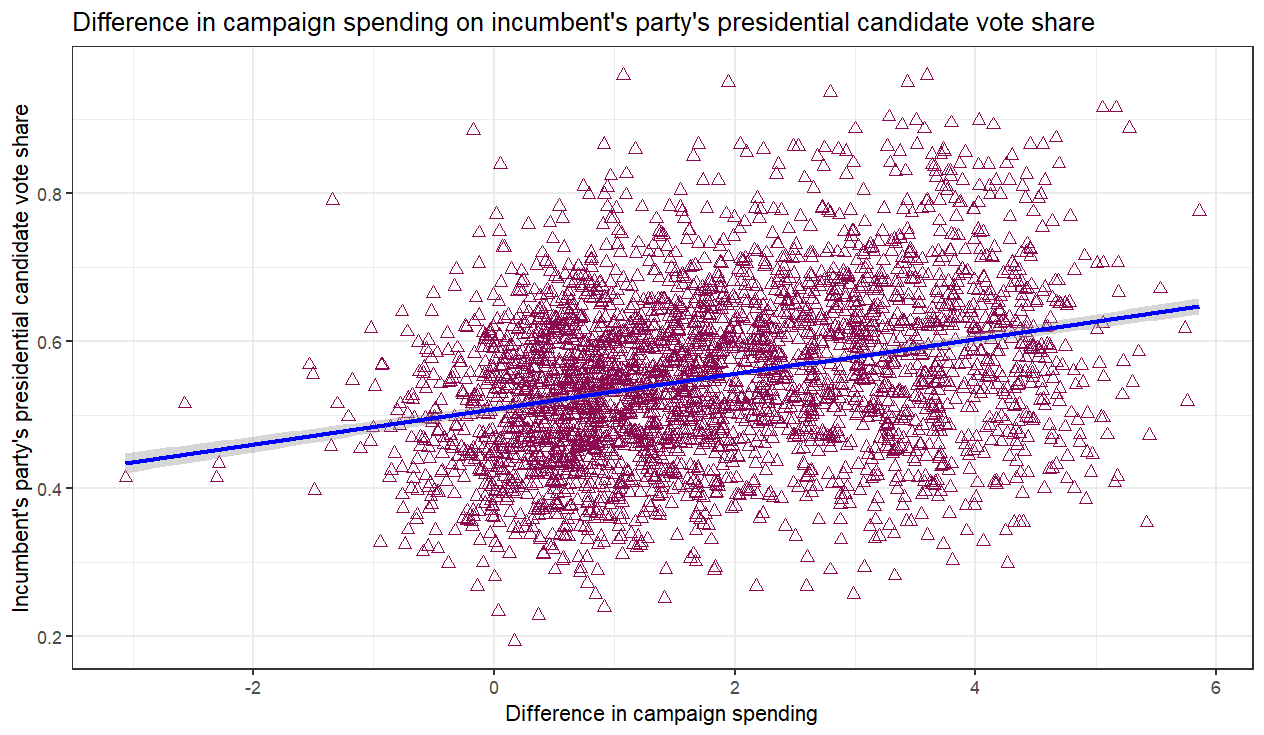
\includegraphics[width=\linewidth]{Rplot2.png}
				\caption{Difference in campaign spending on incumbent's party's presidential candidate vote share.}
				\label{fig:Difference in campaign spending on incumbent's party's presidential candidate vote share}
			\end{figure}
			
			\textit{Interpretation of Figure 2 scatter plot: reflects the findings of the previous regression, a positive linear relationship between both variables. It reflects a positive correlation between both variables. However, the linear relationship appears to be less strong than in Figure 1 - therefore it is not very strong but a correlation exists.}\vspace{.5cm}
				
		
		\item Save the residuals of the model in a separate object.	\vspace{.5cm}
		
			\textbf{code}		
			\begin{verbatim}
				res2 <- resid(reg2)
				res2
			\end{verbatim}
			
			\textit{Residuals indicate the distance of the values of each observation from the predicted values, which fall on the line of best fit.}\vspace{.5cm}
		
		\item Write the prediction equation.
		
		\textit{The formula for the prediction equation is: y = intercept +(slope*x). Therefore, using the data from the regression, the formula for this question is: incumbent party's presidential candidate vote share = 0.507583 + (0.023837*difference in campaign spending).}\vspace{.5cm}
		
	\end{enumerate}
	
	\newpage	
\section*{Question 3}

\noindent We are interested in knowing how the vote share of the presidential candidate of the incumbent's party is associated with the incumbent's electoral success.
	\vspace{.25cm}
	\begin{enumerate}
		
		\item Run a regression where the outcome variable is \texttt{voteshare} and the explanatory variable is \texttt{presvote}.
			\vspace{.5cm}
			
			\textbf{code}		
			\begin{verbatim}
				reg3 <- lm(voteshare ~ presvote, data=inc.sub)
				reg3
				summary(reg3)# inspect results
				stargazer(reg3, title = "Vote share of incumbent party's 
				presidential candidate on on incumbent's electoral success")
				
			\end{verbatim}
			
			\textbf{Stargazer table}		
			
			% Table created by stargazer v.5.2.3 by Marek Hlavac, Social Policy Institute. E-mail: marek.hlavac at gmail.com
			% Date and time: Thu, Nov 13, 2025 - 22:07:43
			\begin{table}[!htbp] \centering 
				\caption{Vote share of incumbent party's presidential candidate on incumbent's electoral success} 
				\label{} 
				\begin{tabular}{@{\extracolsep{5pt}}lc} 
					\\[-1.8ex]\hline 
					\hline \\[-1.8ex] 
					& \multicolumn{1}{c}{\textit{Dependent variable:}} \\ 
					\cline{2-2} 
					\\[-1.8ex] & voteshare \\ 
					\hline \\[-1.8ex] 
					presvote & 0.388$^{***}$ \\ 
					& (0.013) \\ 
					& \\ 
					Constant & 0.441$^{***}$ \\ 
					& (0.008) \\ 
					& \\ 
					\hline \\[-1.8ex] 
					Observations & 3,193 \\ 
					R$^{2}$ & 0.206 \\ 
					Adjusted R$^{2}$ & 0.206 \\ 
					Residual Std. Error & 0.088 (df = 3191) \\ 
					F Statistic & 826.950$^{***}$ (df = 1; 3191) \\ 
					\hline 
					\hline \\[-1.8ex] 
					\textit{Note:}  & \multicolumn{1}{r}{$^{*}$p$<$0.1; $^{**}$p$<$0.05; $^{***}$p$<$0.01} \\ 
				\end{tabular} 
			\end{table} 
			
			\textit{Interpretation of regression: The intercept is 0.441330, the regression coefficient of presvote is 0.388018, representing a positive relationship between both variables, it indicates that as the vote share of the incumbent's party's presidential candidate increases, so does the incumbent's vote share. The p-value is <2e-16, which suggests the probability of obtaining results at least as extreme as those observed, with such a small p-value, we can reject the null hypothesis that there is no relationship between incumbent's party's presidential candidate vote share and incumbent party's presidential candidate's vote share. This would suggest that in a year where an incumbent's party fields a presidential candidate that does well, the incumbent will also do well.}\vspace{.5cm}
			
        \newpage	
			
		\item Make a scatterplot of the two variables and add the regression line. 
			\vspace{.5cm}
			
			\textbf{code}		
			\begin{verbatim}
				ggplot(data=inc.sub, aes(x = presvote, y = voteshare)) +
				geom_point(size = 2, shape = 1) +
				geom_smooth(method = lm, color = "red3") +
				labs(title = "Vote share of incumbent's party's presidential candidate on incumbent's electoral success",
				x = "Incumbent's party's presidential candidate vote share",
				y = "Incumbent vote share") +
				theme_bw()
			\end{verbatim}
			
			\begin{figure}
				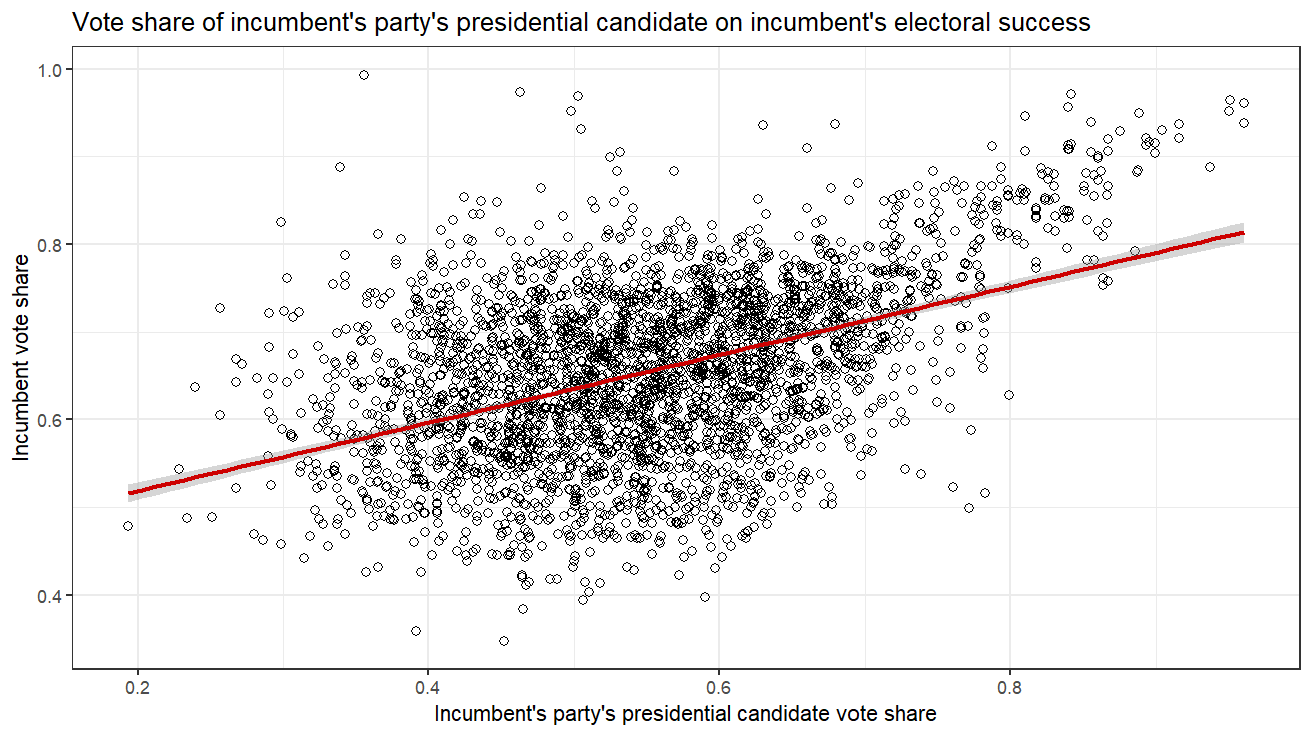
\includegraphics[width=\linewidth]{Rplot3.png}
				\caption{Vote share of incumbent's party's presidential candidate on incumbent's electoral success.}
				\label{fig:Vote share of incumbent's party's presidential candidate on incumbent's electoral success}
			\end{figure}
			
			\textit{Interpretation of Figure 3 scatter plot: reflects the findings of the previous regression, a strong positive linear relationship between both variables. It reflects a positive correlation between both variables. The linear relationship appears to similar to that of Figure 1, however, similar to Figure 2, observations appear to cluster around the centre and skew slightly to the left.}\vspace{.5cm}
			
			\newpage
			
		\item Write the prediction equation.
		
			\textit{The formula for the prediction equation is: y = intercept +(slope*x). Therefore, using the data from the regression, the formula for this question is: incumbent's vote share = 0.579031 + (0.041666*Incumbent's party's presidential candidate vote share).}\vspace{.5cm}
		
	\end{enumerate}
	

\newpage	
\section*{Question 4}
\noindent The residuals from part (a) tell us how much of the variation in \texttt{voteshare} is $not$ explained by the difference in spending between incumbent and challenger. The residuals in part (b) tell us how much of the variation in \texttt{presvote} is $not$ explained by the difference in spending between incumbent and challenger in the district.
	\begin{enumerate}
		\item Run a regression where the outcome variable is the residuals from Question 1 and the explanatory variable is the residuals from Question 2.	\vspace{.6cm}
		
		\textbf{code}		
		\begin{verbatim}
			res_data <- data.frame(res1 = res1, res2 = res2)
			reg4 <- lm(res1 ~ res2)
			summary(reg4)
			stargazer(reg4, title = "Residuals Q2 on residuals of Q1")
			
		\end{verbatim}
		
		\textbf{Stargazer table}		
		
		% Table created by stargazer v.5.2.3 by Marek Hlavac, Social Policy Institute. E-mail: marek.hlavac at gmail.com
		% Date and time: Thu, Nov 13, 2025 - 22:32:52
		\begin{table}[!htbp] \centering 
			\caption{Residuals Q2 on residuals of Q1} 
			\label{} 
			\begin{tabular}{@{\extracolsep{5pt}}lc} 
				\\[-1.8ex]\hline 
				\hline \\[-1.8ex] 
				& \multicolumn{1}{c}{\textit{Dependent variable:}} \\ 
				\cline{2-2} 
				\\[-1.8ex] & res1 \\ 
				\hline \\[-1.8ex] 
				res2 & 0.257$^{***}$ \\ 
				& (0.012) \\ 
				& \\ 
				Constant & $-$0.000 \\ 
				& (0.001) \\ 
				& \\ 
				\hline \\[-1.8ex] 
				Observations & 3,193 \\ 
				R$^{2}$ & 0.130 \\ 
				Adjusted R$^{2}$ & 0.130 \\ 
				Residual Std. Error & 0.073 (df = 3191) \\ 
				F Statistic & 476.975$^{***}$ (df = 1; 3191) \\ 
				\hline 
				\hline \\[-1.8ex] 
				\textit{Note:}  & \multicolumn{1}{r}{$^{*}$p$<$0.1; $^{**}$p$<$0.05; $^{***}$p$<$0.01} \\ 
			\end{tabular} 
		\end{table} 
		
		\textit{Interpretation of regression: The intercept is -5.934e-18, the regression coefficient of residuals from Q2 is 2.569e-01, representing a positive relationship between both variables, it indicates that as the residuals from Q2 increase, so do those from Q1. As residuals capture the difference between the predicted values of each regression and the observed values, the differences represent confounding variables which on average further explain the values of both vote shares.The p-value is <2e-16, which suggests the probability of obtaining results at least as extreme as those observed, with such a small p-value, we can reject the null hypothesis that there is no between both sets of residuals.}\vspace{.5cm}
		
		\newpage		
		
		\item Make a scatterplot of the two residuals and add the regression line. 	\vspace{.6cm}
		
		\textbf{code}		

		\begin{verbatim}
			ggplot(data=res_data, aes(x = res2, y = res1)) +
			geom_point(size = 2, shape = 1) +
			geom_smooth(method = lm, color = "red3") +
			labs(title = "Residuals Q2 on residuals of Q1",
			x = "residuals 2",
			y = "residuals 1") +
			theme_bw()
		\end{verbatim}
		
		\begin{figure}
			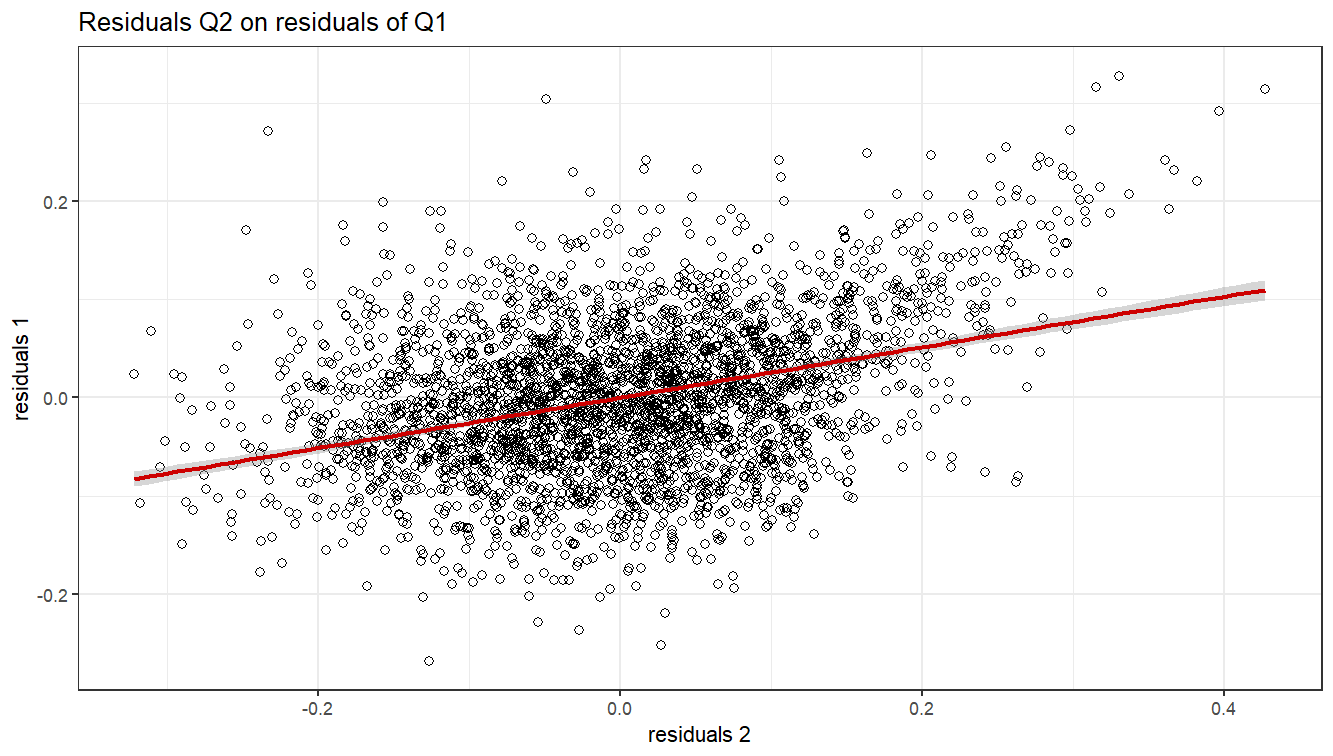
\includegraphics[width=\linewidth]{Rplot4.png}
			\caption{Residuals Q2 on residuals Q1.}
			\label{fig:Residuals Q2 on residuals Q1}
		\end{figure}
		
		\textit{Interpretation of Figure 4 scatter plot: It shows a strong positive linear relationship between both residuals. It reflects a positive correlation between both residuals. Figure 4 strongly resembles Figure 3 - this may indicate a relationship between the residuals of Figure 1 and 2 and Figure 3 - i.e. the difference between the expected values and observed values of both vote shares and difference in campaign expenditure can be explained by the relationship between both vote shares - this is tested in question 5}\vspace{.5cm}
		
		\newpage
		
		\item Write the prediction equation.
		
			\textit{The formula for the prediction equation is: y = intercept +(slope*x). Therefore, using the data from the regression, the formula for this question is: Residuals 1 = -5.934e-18 + (2.569e-01*Residuals 2).}\vspace{.5cm}
		
	\end{enumerate}
	
	\newpage	

\section*{Question 5}
\noindent What if the incumbent's vote share is affected by both the president's popularity and the difference in spending between incumbent and challenger? 
	\begin{enumerate}
		\item Run a regression where the outcome variable is the incumbent's \texttt{voteshare} and the explanatory variables are \texttt{difflog} and \texttt{presvote}.	\vspace{.5cm}
		
		\textbf{code}		
		\begin{verbatim}
			reg5 <- lm(voteshare ~ difflog + presvote, data=inc.sub)
			summary(reg5)
			stargazer(reg5, title = "difflog and presvote on voteshare")
			
		\end{verbatim}
		
		\textbf{Stargazer table}		
		
		% Table created by stargazer v.5.2.3 by Marek Hlavac, Social Policy Institute. E-mail: marek.hlavac at gmail.com
		% Date and time: Thu, Nov 13, 2025 - 22:49:37
		\begin{table}[!htbp] \centering 
			\caption{difflog and presvote on voteshare} 
			\label{} 
			\begin{tabular}{@{\extracolsep{5pt}}lc} 
				\\[-1.8ex]\hline 
				\hline \\[-1.8ex] 
				& \multicolumn{1}{c}{\textit{Dependent variable:}} \\ 
				\cline{2-2} 
				\\[-1.8ex] & voteshare \\ 
				\hline \\[-1.8ex] 
				difflog & 0.036$^{***}$ \\ 
				& (0.001) \\ 
				& \\ 
				presvote & 0.257$^{***}$ \\ 
				& (0.012) \\ 
				& \\ 
				Constant & 0.449$^{***}$ \\ 
				& (0.006) \\ 
				& \\ 
				\hline \\[-1.8ex] 
				Observations & 3,193 \\ 
				R$^{2}$ & 0.450 \\ 
				Adjusted R$^{2}$ & 0.449 \\ 
				Residual Std. Error & 0.073 (df = 3190) \\ 
				F Statistic & 1,302.947$^{***}$ (df = 2; 3190) \\ 
				\hline 
				\hline \\[-1.8ex] 
				\textit{Note:}  & \multicolumn{1}{r}{$^{*}$p$<$0.1; $^{**}$p$<$0.05; $^{***}$p$<$0.01} \\ 
			\end{tabular} 
		\end{table} 
		
		\textit{Interpretation of regression: The intercept is 0.4486442, the regression coefficient of difflog is 0.0355431 and for presvote is 0.2568770 , representing a positive relationship between both explanatory variables on the outcome variable, it indicates that as the difference in campaign expenditure increases and vote share of incumbent's party's presidential candidate increases, so does the incumbent's vote share. However, the relationship appears much stronger between presvote and voteshare.The p-value is <2e-16 for both explanatory variables, which suggests the probability of obtaining results at least as extreme as those observed, with such a small p-value, we can reject the null hypotheses that there is no between both variables and incumbent's vote share.}\vspace{.5cm}
		
		\item Write the prediction equation.	\vspace{.5cm}
		
		\textit{The formula for the prediction equation is: y = intercept + (slope1*x1) + (slope2*x2). Therefore, using the data from the regression, the formula for this question is: Incumbent vote share = 0.4486442 + (0.0355431*difference in campaign spending) + (0.2568770*Incumbent's party's presidential candidate vote share).}\vspace{.5cm}
		
		
		\item What is it in this output that is identical to the output in Question 4? Why do you think this is the case?

			\textbf{code}		
			\begin{verbatim}
				reg5 <- lm(voteshare ~ difflog + presvote, data=inc.sub)
				summary(reg5)
				stargazer(reg5, title = "difflog and presvote on voteshare")
			\end{verbatim}		
		
		% Table created by stargazer v.5.2.3 by Marek Hlavac, Social Policy Institute. E-mail: marek.hlavac at gmail.com
		% Date and time: Thu, Nov 13, 2025 - 23:03:03
		\begin{table}[!htbp] \centering 
			\caption{Results regression 4 and 5} 
			\label{} 
			\begin{tabular}{@{\extracolsep{5pt}}lcc} 
				\\[-1.8ex]\hline 
				\hline \\[-1.8ex] 
				& \multicolumn{2}{c}{\textit{Dependent variable:}} \\ 
				\cline{2-3} 
				\\[-1.8ex] & res1 & voteshare \\ 
				\\[-1.8ex] & (1) & (2)\\ 
				\hline \\[-1.8ex] 
				res2 & 0.257$^{***}$ &  \\ 
				& (0.012) &  \\ 
				& & \\ 
				difflog &  & 0.036$^{***}$ \\ 
				&  & (0.001) \\ 
				& & \\ 
				presvote &  & 0.257$^{***}$ \\ 
				&  & (0.012) \\ 
				& & \\ 
				Constant & $-$0.000 & 0.449$^{***}$ \\ 
				& (0.001) & (0.006) \\ 
				& & \\ 
				\hline \\[-1.8ex] 
				Observations & 3,193 & 3,193 \\ 
				R$^{2}$ & 0.130 & 0.450 \\ 
				Adjusted R$^{2}$ & 0.130 & 0.449 \\ 
				Residual Std. Error & 0.073 (df = 3191) & 0.073 (df = 3190) \\ 
				F Statistic & 476.975$^{***}$ (df = 1; 3191) & 1,302.947$^{***}$ (df = 2; 3190) \\ 
				\hline 
				\hline \\[-1.8ex] 
				\textit{Note:}  & \multicolumn{2}{r}{$^{*}$p$<$0.1; $^{**}$p$<$0.05; $^{***}$p$<$0.01} \\ 
			\end{tabular} 
		\end{table} 
		
		\textit{The coefficient of residuals 2 is 0.257 in regression 4, while the coefficient of presvote is 0.257 in regression 5. This suggests that the variation between observed values in regressions 1 and 2 - where difference in campaign spending is the explanatory variable of both vote shares - can be explained by the relationship between both vote shares. Therefore, the relationship between residuals 1 and 2 is statistically similar to that of presvote on voteshare. This indicates taht where campaign spending differences doesn't explain the variation in vote share for an incumbent/incumbent's party's presidential candidate, the relationship between the presidential candidate's vote share can explain the rise in incumbents vote share. In a country like the US, this can explain the variation in results of incumbent congress members in a presidential election year - where how well their party's candidate does, and how much more they spend than their opponent can affect their ultimate vote share. Notably it suggests that the presidential candidate has a much stronger impact as the coefficient is significantly greater.}
		
		\vspace{.5cm}
		
		\end{enumerate}




\end{document}
